\documentclass[notoc,justified,openany]{tufte-book}    % `notoc` suppresses TL custom TOC, reverts to standard LaTeX
\usepackage{graphicx}
\usepackage{xspace}
\hyphenation{HMMER}
\newcommand{\hmmserver}{\mono{hmmserver}\xspace}
\newcommand{\Hmmserver}{\mono{Hmmserver}\xspace}
\newcommand{\hmmclient}{\mono{hmmclient}\xspace}
\newcommand{\Hmmclient}{\mono{Hmmclient}\xspace}
\newcommand{\hmmpgmd}{\mono{hmmpgmd}\xspace}
\newcommand{\Hmmpgmd}{\mono{Hmmpgmd}\xspace}
\newcommand{\userguide}{HMMER User's Guide}
\input{titlepage_server}                    % definitions for \maketitle 
\bibliographystyle{unsrtnat-brief}   % customized natbib unsrtnat. Abbrev 3+ authors to ``et al.'' 

\begin{document}
\setcounter{tocdepth}{2}             % 0=chapters 1=sections 2=subsections 3=subsubsections? 4=paragraphs
\newcommand{\UNIrelease}{2018\_07}
\newcommand{\UNInseq}{557,992}

\newcommand{\HMMERversion}{3.3dev}
\newcommand{\HMMERdate}{November 2018}

\newcommand{\BGLnseq}{4}
\newcommand{\BGLalen}{171}
\newcommand{\BGLmlen}{149}
\newcommand{\BGLgaps}{22}
\newcommand{\BGLeffn}{0.96}
\newcommand{\BGLre}{0.589}

\newcommand{\HMMERfmtversion}{f}
\newcommand{\HMMERsavestamp}{[3.3dev | November 2018]}

\newcommand{\SGUevalue}{6.8e-65}
\newcommand{\SGUbitscore}{222.7}
\newcommand{\SGUbias}{3.2}
\newcommand{\SGUorigscore}{225.9}
\newcommand{\SGUdombitscore}{222.6}
\newcommand{\SGUseqname}{MYG\_PHYCD}
\newcommand{\SGUmsvpass}{3.8}
\newcommand{\SGUbiaspass}{17573}
\newcommand{\SGUvitpass}{2369}
\newcommand{\SGUfwdpass}{1127}
\newcommand{\SGUelapsed}{9.7}

\newcommand{\SFSevalue}{6.2e-56}
\newcommand{\SFSbitscore}{173.1}
\newcommand{\SFSdomevalue}{1.1e-16}
\newcommand{\SFSdombitscore}{47.3}
\newcommand{\SFSexpdom}{9.5}
\newcommand{\SFSndom}{9}

\newcommand{\SFSmaxdom}{7}
\newcommand{\SFSmaxdomu}{5}
\newcommand{\SFSmaxsc}{47.3}
\newcommand{\SFSievalue}{1.1e-16}
\newcommand{\SFSuievalue}{6.0e-11}
\newcommand{\SFSdomZ}{784}
\newcommand{\SFSucevalue}{8.4e-14}
\newcommand{\SFSaidx}{1}
\newcommand{\SFSascore}{-1.5}
\newcommand{\SFSaevalue}{0.18}
\newcommand{\SFSauevalue}{141}
\newcommand{\SFSacoords}{395-410}
\newcommand{\SFSbidx}{6}
\newcommand{\SFSbscore}{0.6}
\newcommand{\SFSbevalue}{0.04}
\newcommand{\SFSbuevalue}{31.4}
\newcommand{\SFSbcoords}{1720-1769}
\newcommand{\SFSainsig}{5.0}
\newcommand{\SFSbinsig}{10.1}

\newcommand{\JHUninc}{954}
\newcommand{\JHUnsig}{954}

\newcommand{\NMHafrom}{302390}
\newcommand{\NMHato}{302466}
\newcommand{\NMHbfrom}{302466}
\newcommand{\NMHbto}{302389}
\newcommand{\NMHnres}{660000}
\newcommand{\NMHntop}{330000}
\newcommand{\NMHnssv}{76413}
\newcommand{\NMHfracssv}{11.6}
\newcommand{\NMHnbias}{56984}
\newcommand{\NMHfracbias}{8.6}
\newcommand{\NMHnvit}{5675}
\newcommand{\NMHfracvit}{0.9}
\newcommand{\NMHnfwd}{3194}
    % snippets captured from output, by gen-inclusions.py 

\maketitle

\vspace*{\fill}
\begin{flushleft}
@COPYRIGHT@

\vspace{5mm}
Permission is granted to make and distribute verbatim copies of this
manual provided the copyright notice and this permission notice are
retained on all copies.

\vspace{5mm}
HMMER is licensed and freely distributed under the GNU General Public
License (GPL). For a copy of the full text of the GNU General Public
License, see
\htmladdnormallink{www.gnu.org/licenses}{http://www.gnu.org/licenses/}.

\vspace{5mm}
For alternative licensing terms, including commercial licenses,
contact the Office of Technology Management at the Washington
University School of Medicine.

\vspace{5mm}
\end{flushleft}




\begin{adjustwidth}{}{-1in}          % TL \textwidth is quite narrow. Expand it manually for TOC and man pages.
\tableofcontents                     
\end{adjustwidth}


\chapter{Introduction}
\Hmmserver and \hmmclient are replacements for the \hmmpgmd and \mono{hmmc2} programs provided by earlier versions of HMMER.  Like \hmmpgmd, \hmmserver is a persistent, long-running, service that provides high-performance homology searches by caching sequence and HMM databases in RAM and distributing the work of each search across many computers and threads.  \Hmmclient is a full-featured command-line client application for \hmmserver that submits searches to a running server and displays results in a format that is as close as possible to that of the \mono{hmmsearch}, \mono{hmmscan}, \mono{phmmer}, and \mono{jackhmmer} programs.  It is thus a significant upgrade to the \mono{hmmc2} program, which was more of a debugging tool for \hmmpgmd than a full client program.

\Hmmserver improves on \hmmpgmd in several ways:
\begin{enumerate}
\item{Parallelization has been significantly improved.  \Hmmserver uses a work-requesting protcol to distribute work across the machines that make up a server and a combination of work-requesting and work-stealing to balance load across the worker threads on each worker machine.  Together, these parallelization improvements reduce search time by approximately 50\% when the server is run on hundreds of cores.}
\item{\Hmmserver reads standard FASTA and HMM files as its inputs, instead of the special-format files \hmmpgmd requires.  This allows it (at some cost in memory usage) to return the full results of a search.  In contrast, \hmmpgmd replaces the metadata (name, accession, taxonomy ID, etc.) associated with each sequence or HMM in a database with a unique ID, requiring database or file accesses to retrieve that metadata before results can be returned, which has proven to be a significant performance bottleneck.}
\item{\Hmmserver can load multiple sequence and/or HMM databases into memory simultaneously and accept searches to any of them in any order.  In contrast, \hmmpgmd could only load a single sequence or HMM database.  This required users to run separate instances of \hmmpgmd for sequence and HMM data, potentially wasting resources if the fraction of searches to each type of database was not predicted accurately.  Similarly, if a user wanted to provide the ability to search multiple databases of a given data type, they had to either run a separate instance of \hmmpgmd for each database or create a single data file containing all of the data in all of the databases and implement searches of individual databases as searches of sub-ranges of the unified database.  Generating these unifiied databases any time one of the individual databases changed proved to be time-consuming for our partners at the European Bioinformatics Institute (EBI), making it more difficult for them to provide the latest version of each database on their \hmmpgmd server.}
\item{\Hmmserver implements a more-flexible sharding scheme than \hmmpgmd.  Originally, \hmmpgmd required each worker node to load the entire database that \hmmpgmd caches into RAM. As sequence database sizes increased, the amount of RAM this requried became a problem, so \hmmpgmd was modified to shard its database by loading $\frac{1}{N}th$ of the database onto each worker node of a system with N workers.}
\item{\Hmmserver is implemented as an MPI application, in contrast to \hmmclient, which was a set of independent programs that communicated via UNIX sockets.  This allows \hmmserver to take advantage of high-bandwidth computer networks to improve performance, and simplifies the process of starting an \hmmserver, as the entire server can be started as a single MPI application across multiple machines.}
\end{enumerate}



\chapter{Installation}
\Hmmserver and \hmmclient are included in the standard HMMER distribution package, but HMMER must be compiled with MPI support turned on for \hmmserver to be useful, so it is likely you will have to compile HMMER from source to use the server.  Builds of HMMER without MPI support enabled will create a \hmmserver executable, which will print an error message and exit if run.  \Hmmclient does not require MPI support, so any installation of HMMER should have a working \hmmclient application.

To build HMMER with MPI support, obtain a source-code copy of HMMER from hmmer.org\sidenote{The \userguide has more detail on how to do this.} or elsewhere and go through the standard configuration/build process, with one change: you must pass the \mono{--enable-mpi} flag to our configure script to cause HMMER to be built with MPI support:

\vspace{1ex}
\user{\% ./configure {-}{-}prefix=/your/install/path {-}{-}enable-mpi}\\
\vspace{1ex}

After configuring the build to enable MPI, running \mono{make} as normal will build HMMER with MPI support and create a functional \hmmserver program.  One note, however, is that building HMMER in this way will make all of our programs dependent on the MPI libraries.  If your system (like the one we develop on) requires the user to take steps to make the MPI libraries available, you may find it more convenient to build most of HMMER without MPI support, do a separate build with MPI support enabled, and copy the \hmmserver executable from the MPI-enabled build to the non-MPI build so that it is the only application that loads the MPI libraries.

Once HMMER has been built, \hmmserver and \hmmclient will be available in the \mono{src} directory of the distribution, and can either be run from there or made available system wide by running \mono{make install}.


\chapter{Usage}

\section{Hmmserver}
\Hmmserver must be run as an MPI process with at least one rank for the master node and one worker rank for each shard that the target database(s) will be divided into.  The different implementations of MPI vary in how this is done, but a common invocation of \hmmserver would be\sidenote{On many systems, MPI jobs need to be sumbitted through a job control mechanism such as SLURM.  See your system documentation for information on how to use the job control system on your cluster.}:

\vspace{1ex}
\user{\% mpirun {-}n <number of ranks> hmmserver {-}num\_dbs <n>}\\
\vspace{1ex}

One challenge that comes from making \hmmserver an MPI process is that the master node of the \hmmserver will run as rank 0 of the MPI process, but the MPI runtime assigns ranks to hosts in an unpredictable manner.  To address this, the master node of \hmmserver determines the host name of its machine and outputs that to standard output at the beginning of execution.  Alternately, the {-}{-}host option to mpirun/mpiexec can be used to specify the set of computers that \hmmserver will run on, and rank 0 will run on the first computer in that list\sidenote{This may be an implementation-dependent behavior.  The documentation for many MPI implementations states that this is what will happen, but we do not believe that this is a required behavior for all implementations of MPI.}

One key decision when starting an \hmmserver is the number of shards (pieces) that each database will be divided into.  In an \hmmserver with $s$ shards, each worker node will load $frac{1}{sth}$ of each database into memory, but will then only be able to process the parts of each search that corresponds to the items it has in RAM.  This creates a tradeoff between performance and memory requirements: increasing the number of shards a server uses will decrease the amount of memory used on each worker node, but will reduce performance by restricting the set of nodes that each shard's fraction of the search can be distributed across.  While the only hard requirement is that the number of worker nodes must be at least equal to the number of shards, using a number of shards that is not an integer divisor of the number of worker nodes will reduce performance by having one or more shards with fewer nodes assigned to them than others. For example, a server with eight worker nodes could be set to divide its databases into three shards, but this would result in two of the shards having three worker nodes assigned to them, and one shard only having two, in which case the shard with two worker nodes would generally take longer to search than the other two, making it the bottleneck on performance.

Once started, \hmmserver will continue running until it receives a shutdown command from a client, at which point it will terminate.  As an (admittedly weak) protection against spurious/malicious shutdown requests, the \mono{{-}{-}password} option to \hmmserver can be used to specify a password that must be sent along with a shutdown command for the command to take effect.


\section{Hmmclient}
The \hmmclient application provides a command-line interface to send searches to a running \hmmserver and display results in the same manner as the \mono{hmmsearch}, \mono{hmmscan}, \mono{phmmer}, and \mono{jackhmmer} programs.  A typical use of \hmmclient is:

\vspace{1ex}
\user{\% hmmclient {-}s <servername> {-}{-}db <d> <name of the file containing the sequence(s) or HMM(s) to be searched>}\\
\vspace{1ex}
 
\Hmmclient accepts the same set of command-line options for controlling output, managing the acceleration pipeline, defining how HMMs are constructed from sequences, and setting reporting thresholds as \mono{hmmsearch}, \mono{phmmer}, \mono{hmmscan}, and \mono{jackhmmer}.  See the documentation for those programs for more information on those options.  \Hmmclient does not support the \mono{--cpu} option that sets the number of worker threads in our command-line applications, as that decision is made at the time the server is started.

\Hmmclient accepts three types of query objects: HMMs, protein sequences, and multiple-sequence alignments (MSAs).  HMMs and protein sequence queries are sent directly to the server, while MSA queries are converted into HMMs before being sent to the server.

Like our other programs, query objects may either be read from files, or from standard input if a dash ('-') is passed as the name of the query file.  \Hmmclient expects HMM queries to be in .hmm file format, either text-mode or processed with \mono{hmmpress}.  It accepts sequence queries in {FASTA}, {UniProt}, {Genbank}, {DDBJ} and {EMBL} formats, and multiple-sequence alignment queries in Stockholm, aligned {FASTA}, {CLUSTAL}, interleaved {PHYLIP}, and {SELEX} formats\sidenote{See the files esl\_sqio.tex and esl\_msafile.md in your Easel distribution for more detail on sequence and MSA file formats.}.

Accepting this wide a range of query formats means that, unlike many of our other programs, \hmmclient cannot determine the type of query object it has been passed by examining the contents of the query file\sidenote{One reason that this is necessary is that our routines that read sequence files treat MSA files as sets of unaligned sequenvces.}.  \Hmmclient defaults to assuming its query is as HMM unless the \mono{{-}{-}qseq} option is specified to indicate that the query file contains seqences or the \mono{{-}{-}qmsa} option is passed to indicate that the query file contains multiple-sequence alignments.  In most cases, \hmmclient can automatically determine the format of the query file once it knows the type of the query object.  When that is not possible, the \mono{{-}{-}qformat <format>} command can be used to explicitly specify the format of the query file.

A query file may contain one or more query objects.  \Hmmclient reads each query object from a file sequentially and submits a separate query to the server for each object.  

\Hmmclient also supports iterative (\mono{jackhmmer}-style) queries.  To instruct \hmmclient to perform an iterative query, pass the \mono{{-}{-}jack <maxrounds>} option on the command line, where \mono{<maxrounds>} specifies the maximum number of iterative queries that should be done if the query does not converge before then.  \Hmmclient only supports iterative queries when the query object is one or more sequences.

In addition to queries, \hmmclient can send two instructions to the server.  The first, specified by passing \mono{{-}{-}contents} on the command line, instructs the server to return a list of the databases that it has available to be searched.  The second, specified by passing \mono{{-}{-}shutdown} on the command line, instructs the server to shut down.  A shutdown instruction may also specify a password, indicated by the \mono{{-}{-}password <password>} flag on the command line. If the server has been configured to require a password to shut down, a shutdown instruction must provide a matching password, otherwise an error will occur. Each invocation of \hmmclient can either send one instruction or one or more queries to the server; attempting to send two instructions or an instruction and one or more queries in the same invocation results in an error.

\chapter{For those converting from an hmmpgmd installation}
For an administrator, the biggest change between \hmmpgmd and \hmmserver is the switch from independent programs to an MPI application.  This allows \hmmserver to be started with a single command, although the exact syntax of this command may vary between implementations of MPI.  See your local system documentation for more information.

Making \hmmserver an MPI application introduces the challenge of determining what machine the master rank (rank 0) of the server is running on, and thus which machine clients should send queries to.  There are two ways to do this.  The first is to examine the output of \hmmserver shortly after the server starts, as the master rank will print its hostname on standard out.  The second is to use options to the command that starts \hmmserver, such as the \mono{--host} flag supported by many MPI implementations, to control which machines \hmmserver runs on and thus specify the machine that will run the master rank.

We attempted to keep the client interface to \hmmserver as close as possible to that of \hmmpgmd, but a few changes were necessary.  The two most significant of these are:
\begin{itemize}
  \item{\Hmmserver only allows a client to send one query to the server per socket connection, requiring that the client disconnect from the server after each search completes and request a new connection if it wants to send another request.  In contrast, \hmmpgmd allowed a client to open a socket connection and send multiple query requests before disconnecting, which, in some cases, led to clients monopolizing the server by sending large numbers of requests in one connection.  Requiring a client to disconnect and reconnect between queries forces it to arbitrate with other clients for use of the server, making it harder for one poorly-behaved client to lock others out of the server.}
  \item{\Hmmpgmd used two forward slash characters ("//") to indicate the end of a command, which worked because it only accepted text-formatted HMMs and sequences.  \Hmmserver also accepts HMMs as serialized \mono{P7\_HMM} structures, in order to support iterative search without the precision loss that converting an HMM to text format incurse.  To support this, \hmmserver requires two socket messages to transmit a command: one 32-bit message containing the length of the command being sent, followed by the command itself.}  
\end{itemize}



\chapter{Hmmserver's Design}
\Hmmserver is an MPI application that uses a conventional master-worker topology, as shown in Figure \ref{fig:server}.  While the most-common use of \hmmserver will distribute the MPI ranks across multiple machines, this is not required\sidenote{If each MPI rank is not assigned to a separate computer, we strongly recommend using the \mono{--cpu} flag to specify the number of worker threads on each worker rank.  If this is not done, each worker rank will start as many worker threads as its machine has hardware thread slots, severely over-subscribing the hardware if multiple worker ranks run on the same machine.}.  One MPI rank (rank 0) acts as the master rank, while the rest act as workers.  The master rank handles communication with clients, receiving search requests from them and sending results back when each search completes.  The master rank also co-ordinates the work of the workers, assigning them regions of the target database to search and collecting the hits that each worker finds into a single list.  Worker ranks cache the server's target databases in memory and perform the work of each search, and can require significant memory, depending on the number and size of the target databases and the number of shards those databases are divided into.  The master rank does not cache target databases, as it only needs to know the number of items in each database to distribute work across the worker ranks.  Thus, it uses very little memory when the server is idle, but it may require significant amounts of memory to assemble the results of searches that return large numbers of hits.
\begin{figure*}
  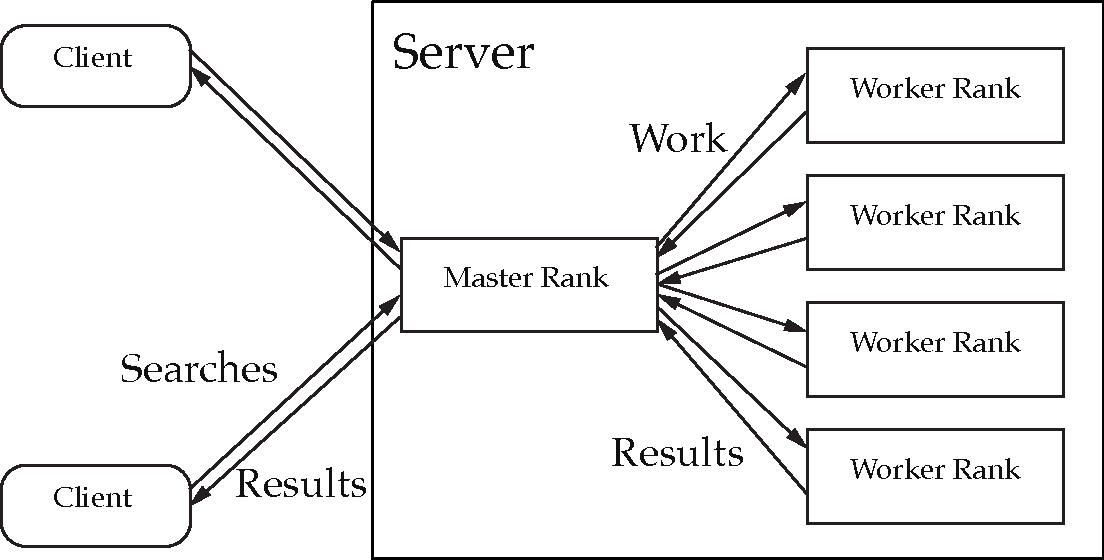
\includegraphics[width=\textwidth]{inclusions/server.pdf}
  \caption{Hmmserver Architecture}
  \label{fig:server}
  \end{figure*} 
The decision to build \hmmserver as an MPI application was a significant change from \hmmpgmd, which was implemented as a set of independent programs that communicate with each other via UNIX sockets.  The initial motivation for this change was to improve performance by taking advantage of high-bandwidth networks, which MPI typically does and sockets typically does not.  During discussions with our collaborators at the European Bioinformatics Institute, they disclosed that managing \hmmpgmd's independent programs was a source of difficulty for them, so the switch to an MPI application provided a second benefit.

\section{Parallelization and Load Balancing}
\Hmmpgmd statically distributed the work of each search across the worker nodes, assigning $\frac{1}{Nth}$ of the items to be searched to each worker node in a system with N workers.  This led to significant variance in the amount of time each worker took to perform its fraction of the search, reducing search performance. The root cause of this load imbalance is the fact that the amount of time to perform a sequence-HMM comparison varies greatly depending on whether the sequence and HMM are clearly not homologs, are close to being similar enough to be considered homologs, or are detected as homologs.  This causes regions of the database that contain many homologs to take much longer to search than regions that contain few homologs.  Thus, worker nodes that find many homologs take significantly longer to finish their fraction of a search than worker nodes that find few homologs.  Worse yet, the distribution of homologs across the target database varies from search to search, making it impossible to find a static allocation of work to worker nodes that balances load well.

To address this, \hmmserver dynamically distributes work across its worker node using a work-requesting system.  The master node maintains a global list of the items in each shard that still need to be compared to complete the search.  Worker nodes each maintain a local list of work (items to be searched) that they are responsible for.  When the amount of work remaining on a worker node's local list drops below a threshold, it sends a request to the master node for more work.  If the master node has any work remaining on its global list, it responds with a chunk of work (range of items) that the worker node is now responsible for.  To trade-off load balancing against the amount of communication required, work chunks contain a large amount of work at the beginning of a search and decrease in size over the course of the search.

\subsection{Within-Node Parallelization}
Within each worker node, \hmmpgmd uses a load-balancing system similar to how \hmmserver distributes work across nodes.  Each worker node maintains a list of the work assigned to it, and worker threads request chunks of work from the list as they complete their previously-assigned work.  This creates a trade-off between load balancing and contention for the work list: if the work chunks are too small, the worker threads need to request more work frequently, and access to the work list becomes a bottleneck.  On the other hand, if the work chunks are too large, the worker thread that grabs the last chunk of work from the list can wind up working for a significant amount of time after the other threads finish, increasing the time to complete each search.

\Hmmserver improves load-balancing by adding work stealing to \hmmpgmd's within-node load balancing scheme.  When a worker thread finds that the work list is empty, it examines the chunks of work that the other worker threads are working on and takes half of the work from the thread with the most to do.  This spreads the work at the end of a search more-evenly across the worker threads, preventing one thread from significantly delaying the end of the search.

\Hmmserver also adds split-phase processing of sequence-HMM comparisons to further improve performance.  The final steps of hit and domain detection can take a significant amount of time, such that the threads processing the last few hits in a search can delay completion noticeably, particularly when running the server on a large enough number of machines to meet our one second average search time goal\sidenote{This was definitely true in the HMMER4 performance prototype of the server, as HMMER4's final stage trades run time for accuracy in some cases.  We have not done a great deal of analysis on whether it is true in HMMER3.}.  To address this, the server splits sequence-HMM comparisons into "front-end" (the filter pipeline) and "back-end" (the main stage) processing.  Initially, all of the worker threads start processing the front end of comparisons.  When a comparison passes all of the steps in the front end, it is placed in a queue for back-end processing, and one of the worker threads is switched to process comparisons out of the back-end queue.  If the depth of the back-end queue exceeds a threshold, additional worker threads are switched to processing the back end of comparisons.  Similarly, if the back-end queue drops below a depth threshold, worker threads are switched back to processing the front end of comparisons.  This has the effect of prioritizing the back-end comparisons that take the longest to handle, decreasing the chance that a small number of long-running comparisons extend the overall search time.


\section{Sharding}
In the database community, \emph{sharding} a database is the practice of dividing the data in a database across multiple computers, reducing the amount of storage required on each computer at the cost of requiring communication between computers when a database query needs to access data that is stored on multiple machines.  In homology search, we use the term the same way, although, since each sequence-HMM comparison in a homology search is independent, sharding a database across multiple machines does not introduce extra communication.  Instead, it restricts the server's ability to distribute work across multiple computers, since only some of the computers now have access to each sequence or HMM.

The initial version of \hmmpgmd did not support sharding, instead requiring that the entire contents of the database file be loaded into memory on each worker node.  As the size of sequence databases increased, the amount of memory this required on each node became a significant problem, so a simple version of sharding was added to \hmmpgmd.  This scheme always divided the database into as many shards as there were worker nodes, distributing the items in the database round-robin across the worker nodes.  This minimized the amount of memory required per worker node, and, since \hmmpgmd statically allocated the work of each search to worker nodes, did not reduce performance.

\Hmmserver supports a more-flexible sharding scheme which, in combination with its improved load-balancing across nodes, allows the user to trade-off memory usage against performance.  \Hmmserver allows the user to specify the number of shards that the database will be divided into independently of the number of worker nodes as long as there is at least one worker node per shard.  If the server has more worker nodes per shard, it loads each shard onto multiple shards and dynamically distributes the work of searching the shard across the nodes that have it loaded into memory.  For example, a server with six worker nodes could be configured with one shard to deliver maximal performance, with six shards to minimize memory usage, or with two or three shards to provide greater performance than the six-shard case at lower memory usage than the one-shard case.  Note that, while server will operate correctly if the number of shards is not an integer divisor of the number of worker nodes, this will lead to reduced performance because some shards will have fewer nodes assigned to them than others.

\section{Client-Server Interface}
Figure \ref{fig:server_interface} shows the sequence of events involved in sending a search request to a \hmmserver and receiving results back.  A client initiates a search request by opening a socket connection to the server.  It then sends a 32-bit message to the server containing the length of the command that will be sent, followed by the command itself.  After the server completes the search, it sends a fixed-length serialized {HMMD\_SEARCH\_STATUS} object back to the client, followed by a {HMMD\_SEARCH\_STATS} object and one {P7\_HIT} object for each hit the search found.  The server then calls the shutdown function on its side of the socket to signal its intent to close the socket.  Once the client has received all of the data, it closes the socket from its end, which, in turn, signals the server to close its end of the socket connection\sidenote{The server will also close its end of the socket if a timeout (default 30 seconds) expires after it executes the socket shutdown operation, to prevent clients from leaving the socket connection open indefinitely.}, at which point the server is ready to accept another search request.

\begin{figure*}
  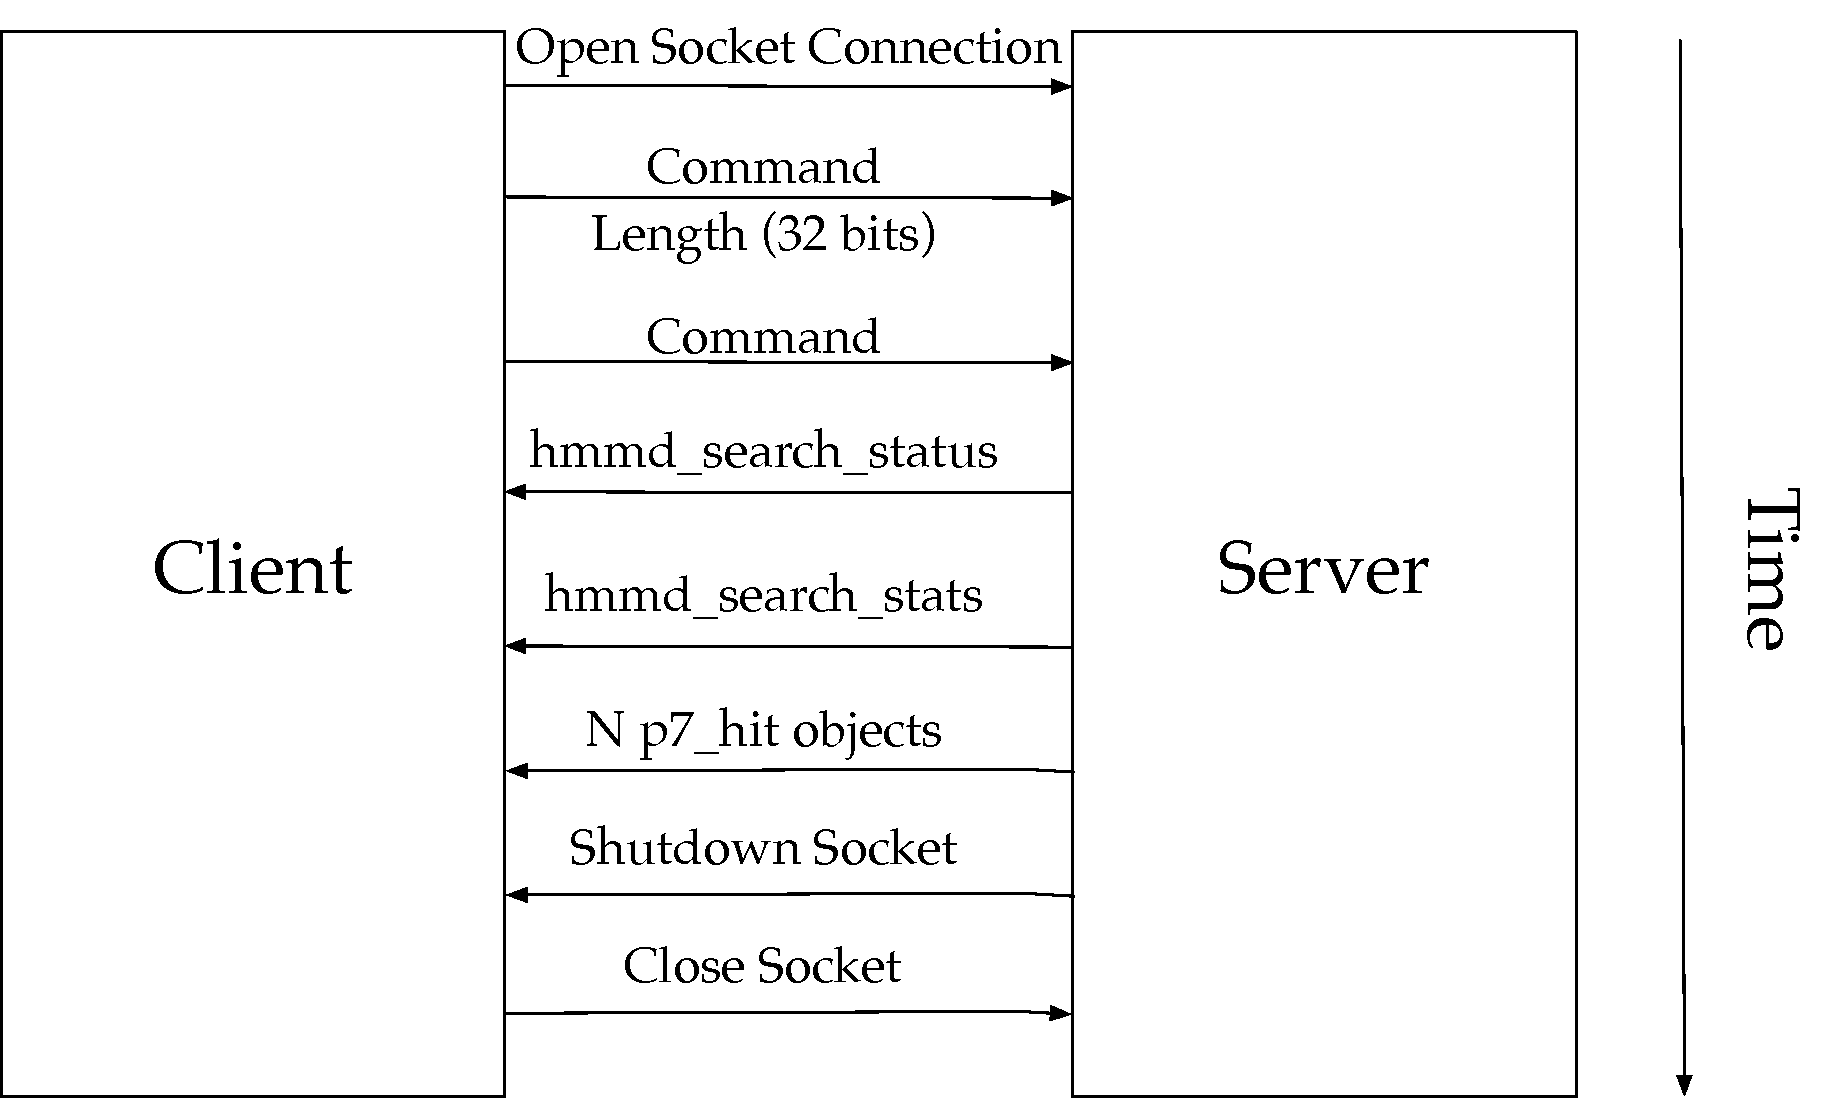
\includegraphics[width=\textwidth]{inclusions/server_interface.pdf}
  \caption{Client-Server Interface}
  \label{fig:server_interface}
  \end{figure*} 

The server can accept multiple client connections simultaneously, up to the limit set by the \mono{{-}{-}ccnts} flag passed to \hmmserver, but queues the requests from clients and processes them sequentially.  Limiting each client to one search per socket connection is new in \hmmserver, as \hmmclient allowed a client to keep a single socket connection open while it sent multiple search requests over the connection.  This change was made to make it harder for clients to monopolize a server.  In \hmmpgmd, a client could potentially send thousands of requests over a single connection.  With \hmmserver, clients can still send many requests to a server, but having to drop and re-establish the socket connection between searches gives other clients a chance to access the server as well.  Note that this "one search per connection" rule applies even to \mono{jackhmmer}-style searches.  \Hmmserver does not implement multi-round searches internally.  Instead a client must send a search request, use the results to create a query object for the next search, send that search, and so on.

\section{Command Format}
Commands are variable-length objects that must begin with a line of ASCII text.  The server accepts two types of commands: search requests and server instructions.

The first line of a search request must begin with the sequence \monob{@-{}-db <database \#>}\sidenote{For backwards compatibility, the server also accepts \monob{@-{}-seqdb <database \#>} and \monob{@-{}-hmmdb <database \#>} as the beginning of a search command, treating them as synonyms for \monob{@-{}-db <database \#>}.}, followed an options string containing the options to be passed by the search.  The second and following lines of a search request contain the query object that will be searched against the specified database, which must either be a FASTA-format sequence, a text-format HMM, or an asterisk followed serialized \mono{{P7\_HMM}} object\sidenote{The server examines the initial character of the query object to determine its format, and the asterisk indicates a serialized \mono{{P7\_HMM}}.}

The following is an example of a search request command. The trailing slash characters are not strictly necessary, but are accepted for compatibility with \hmmpgmd.\\
\vspace{1ex}
\user{\ @{-}{-}db 1  {-}{-}max -Z 42 \\
>sp|Q6GZX3|002L\_FRG3G Uncharacterized protein 002L OS=Frog virus 3 (isolate Goorha)\\
MSIIGATRLQNDKSDTYSAGPCYAGGCSAFTPRGTCGKDWDLGEQTCASGFCTSQPLCAR\\
IKKTQVCGLRYSSKGKDPLVSAEWDSRGAPYVRCTYDADLIDTQAQVDQFVSMFGESPSL\\
AERYCMRGVKNTAGELVSRVSSDADPAGGWCRKWYSAHRGPDQDAALGSFCIKNPGAADC\\
KCINRASDPVYQKVKTLHAYPDQCWYVPCAADVGELKMGTQRDTPTNCPTQVCQIVFNML\\
DDGSVTMDDVKNTINCDFSKYVPPPPPPKPTPPTPPTPPTPPTPPTPPTPPTPRPVHNRK\\
VMFFVAGAVLVAILISTVRW\\
\slash\slash}\\
\vspace{1ex}

\Hmmserver determines the type of search to be performed from the types of the query object and target database, constructing an HMM from the query sequence if both the query object and target database are sequences.  \Hmmserver does not directly support iterative (\mono{jackhmmer}-style) searches.  Instead, the client must send the initial search to the server, construct an HMM from the results, and repeat as necessary.  Support for serialized \mono{{P7\_HMM}} query objects is new in \hmmserver, and was added to support iterative search.  Converting a \mono{{P7\_HMM}} data structure into a text-mode HMM causes some loss of precision because the HMM file format uses a fixed number of digits for each floating-point value, which causes differences in output between iterative searches with \hmmserver and \mono{jackhmmer}.  Sending the HMM for each search round as a serialized data structure eliminates this problem.

Server instructions begin with an exclamation point, followed by the instruction and any arguments.  \Hmmserver currently accepts two instructions.  The first is a request for the server's contents, which has the following format:
\vspace{1ex}
\user{\ !contents}\\
\vspace{1ex}

The second instructs the server to shut down, and has the following format, where the optional password must match the one specified at server startup (if one was specified):\\
\vspace{1ex}
\user{\ !shutdown <optional password>}\\
\vspace{1ex}

\section{Reply Format}
When a \hmmserver completes a search, it sends a serialized\sidenote{Functions to serialize all relevant data structures into network-order streams of bytes and to de-serialize them into big- or little-endian values depending on the endianness of the hardware {HMMER} is running on are provided in the {HMMER} source code.} {HMMD\_SEARCH\_STATUS} object, as shown in Figure \ref{fig:search-status-serialize}, back to the client.  The status field of the object contains an Easel result code, which is either {ESLok} if the search completed correctly, or an error code if something went wrong.  The type field of the object is either {HMMD\_CMD\_SEARCH} or {HMMD\_CMD\_SCAN} depending on whether the target database contained sequence or HMM data.  Finally, the msg\_size field contains the length (in bytes) of the remaining data that will be sent to the client.

  \begin{figure*}
    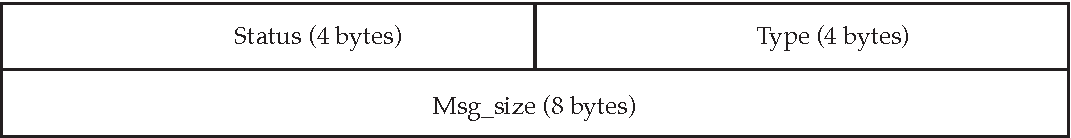
\includegraphics[width=\textwidth]{inclusions/HMMD_SEARCH_STATUS.pdf}
    \caption{Serialized {HMMD\_SEARCH\_STATUS} Structure}
    \label{fig:search-status-serialize}
    \end{figure*} 

If an error occurred during the search, the server then sends a string describing the error.  If the search completed successfully, it sends a serialized {HMMD\_SEARCH\_STATS} structure (Figure \ref{fig:search-stats-serialize}) followed by $N$ serialized {P7\_HIT} structures, one for each hit found by the search.  If an error occurred, the msg\_size field of the {HMMD\_SEARCH\_STATUS} object contains the length of the error description string.  Otherwise it contains the sum of the length of the {HMMD\_SEARCH\_STATS} structure and the $N$ {P7\_HIT} structures, which can be read into a single buffer and un-packed using the deserialization functions HMMER provides.


\begin{figure*}
  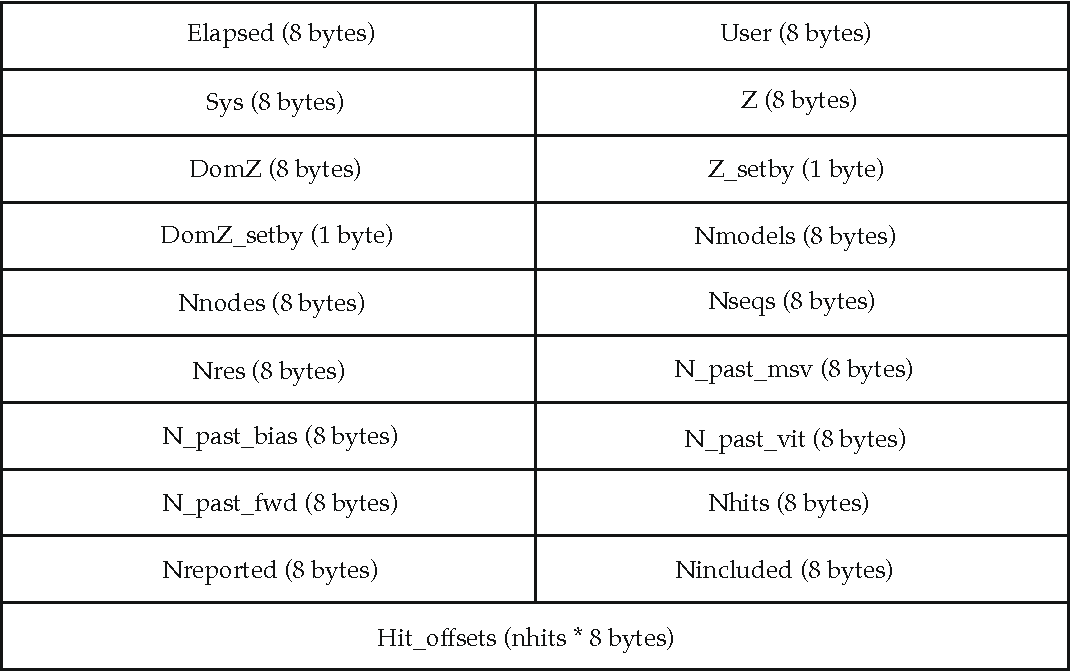
\includegraphics[width=\textwidth]{inclusions/HMMD_SEARCH_STATS.pdf}
  \caption{Serialized {HMMD\_SEARCH\_STATS} Structure}
  \label{fig:search-stats-serialize}
  \end{figure*} 

The {HMMD\_SEARCH\_STATS} structure contains information about the search itself.  The first three fields (elapsed, user, and sys) contain the elapsed, user, and system time required for the search, in seconds, and are double-precision floating-point numbers.  The next four ({Z}, dom{Z}, {Z}\_setby, and dom{Z}\_setby) contain the number of targets searched and number of significant targets searched, which are used in calculating e-values, as well as enums that describe whether the number of targets was set by the database size or a command-line parameter\sidenote{Because the mapping of enums to binary values is not guaranteed to be portable, our serialization and de-serialization routines explicitly convert enums to and from specific integers rather than serializing the actual enums.}. The four fields after than (nmodels, nnodes, nseqs, and nres) contain the number of HMMs searched, number of HMM nodes searched, number of sequences searched, and total number of sequence residues searched.  The next four fields (n\_past\_msv, n\_past\_bias, n\_past\_vit, n\_past\_fwd) contain the number of sequence-HMM comparisons that made it past each of the stages of HMMER's comparison pipeline during the search, and the three after that (nhits, nreported, nincluded) contain the number of hits found, the number of hits that met the reporting threshold for the search, and the number of hits that met the threshold to be considered significant.  Finally, the hit\_offsets array contains the offset (in bytes) from the start of the serialized {P7\_HIT} objects to the start of each {P7\_HIT} objects, if at least one hit was found.

  \begin{figure*}
    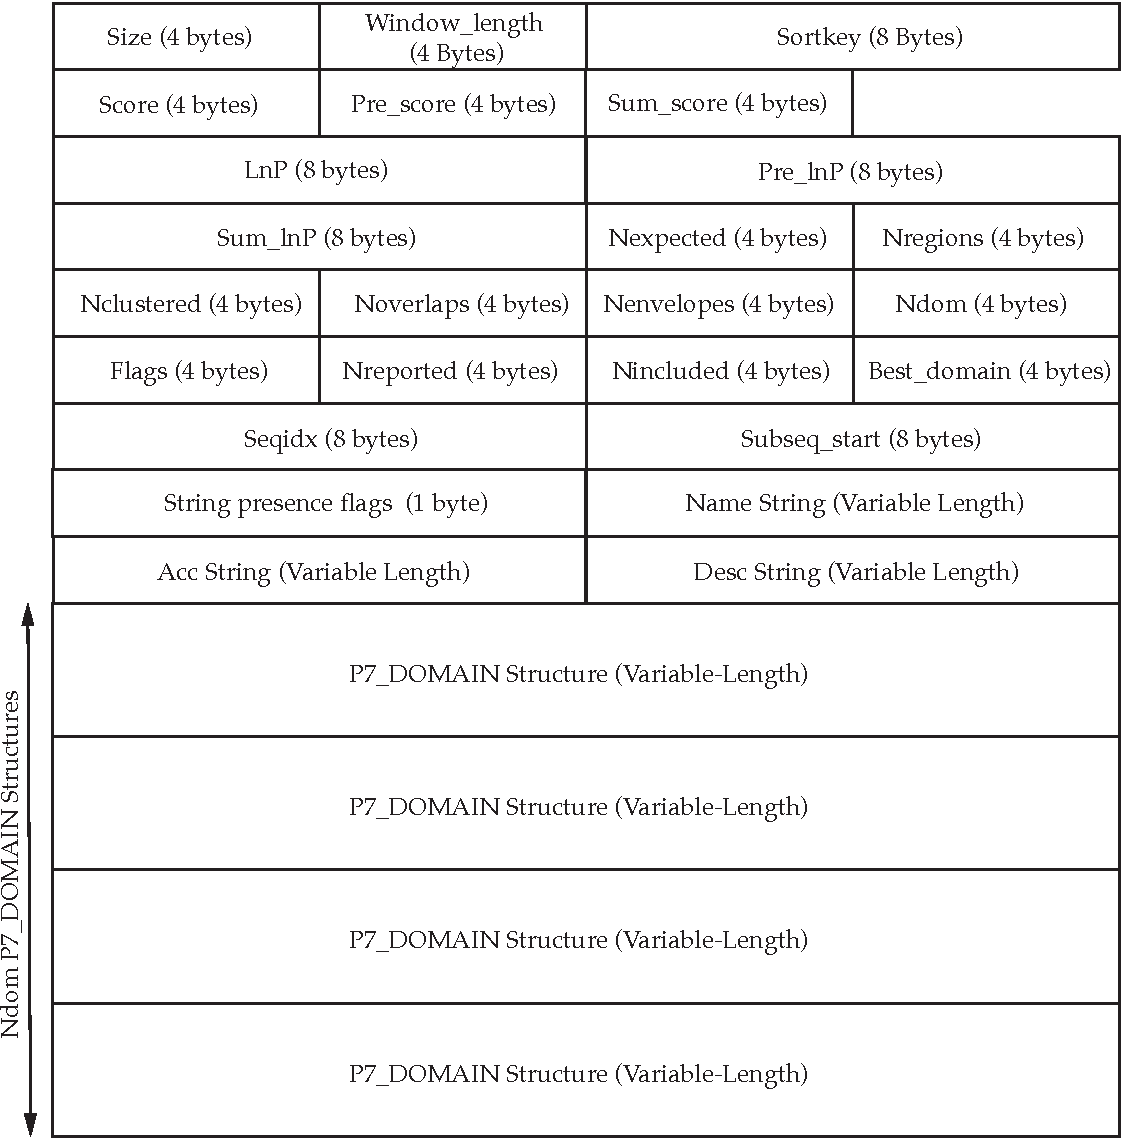
\includegraphics[width=\textwidth]{inclusions/hit-serialize.pdf}
    \caption{Serialized {P7\_HIT} Structures}
    \label{fig:hit-serialize}
  \end{figure*}

  {P7\_HIT} objects, shown in Figure \ref{fig:hit-serialize} are somewhat complex to serialize and de-serialize, as they are variable-length themselves, have optional fields, and contain {P7\_DOMAIN} structures, which contain {P7\_ALIDISPLAY} structures, both of which are variable-length.  Because of the number of fields in these data structures, we refer the reader to the {HMMER} source code for information about the meaning of each data structure's fields, and only describe here how the serialization of these data structures differs from a straightforward concatenation of the fields in the structure into a network-ordered stream of bytes.

  A serialized {P7\_HIT} structure begins with a four-byte size field that is not part of the {P7\_HIT} structure and contains the length (in bytes)
  of the serialized {P7\_HIT} object.  This is followed by all of the fixed-length fields in the data structure, a one-byte field of string presence flags that encode whether the {P7\_HIT} object contains the optional acc and desc strings, and the variable-length name acc, and desc strings (if present) from the {P7\_HIT} object.  The serialized object then concludes with $Ndom$ serialized {P7\_DOMAIN} structures.

  \begin{figure*}
    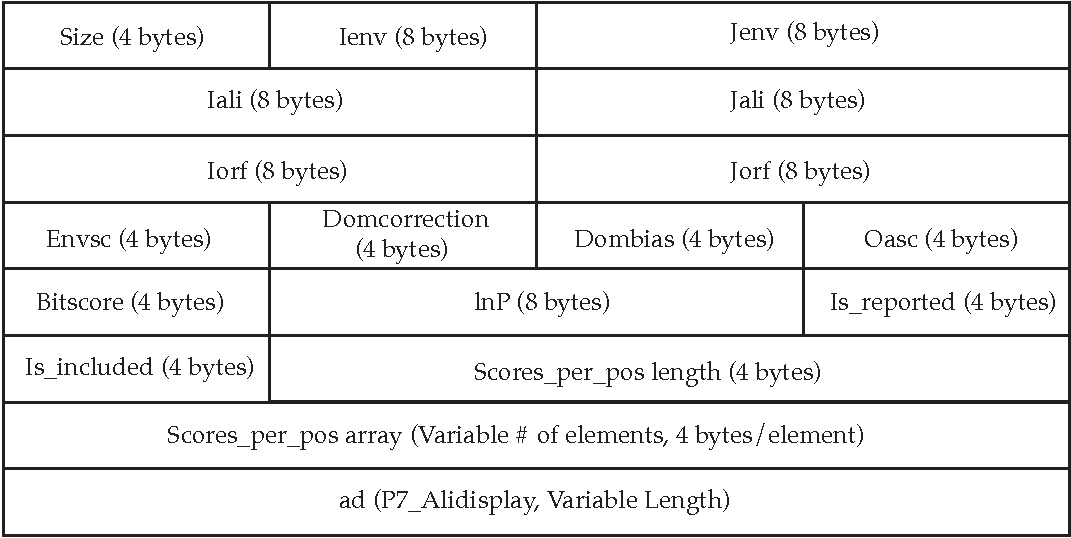
\includegraphics[width=\textwidth]{inclusions/domain-serialize.pdf}
    \caption{Serialized {P7\_DOMAIN} Structure}
    \label{fig:domain-serialize}
  \end{figure*}

  The {P7\_DOMAIN} structure (Figure \ref{fig:domain-serialize}) is relatively straightforward to serialize.  The serialized structure begins with a size field that encodes its length in bytes, followed by the fixed-length fields of the data structure.  The only complexity comes from the scores\_per\_pos array, which is a variable-length array of floating-point numbers.  The scores\_per\_pos length field\sidenote{This field is not strictly necessary, as it contains the same information as the n field of the domain's {P7\_ALIDISPLAY} structure, but including it explicitly simplifies de-serialization.} gives the length of this array in elements, and is followed by the serialized scores\_per\_pos array and the domain's {P7\_ALIDISPLAY} structure.
  \begin{figure*}
    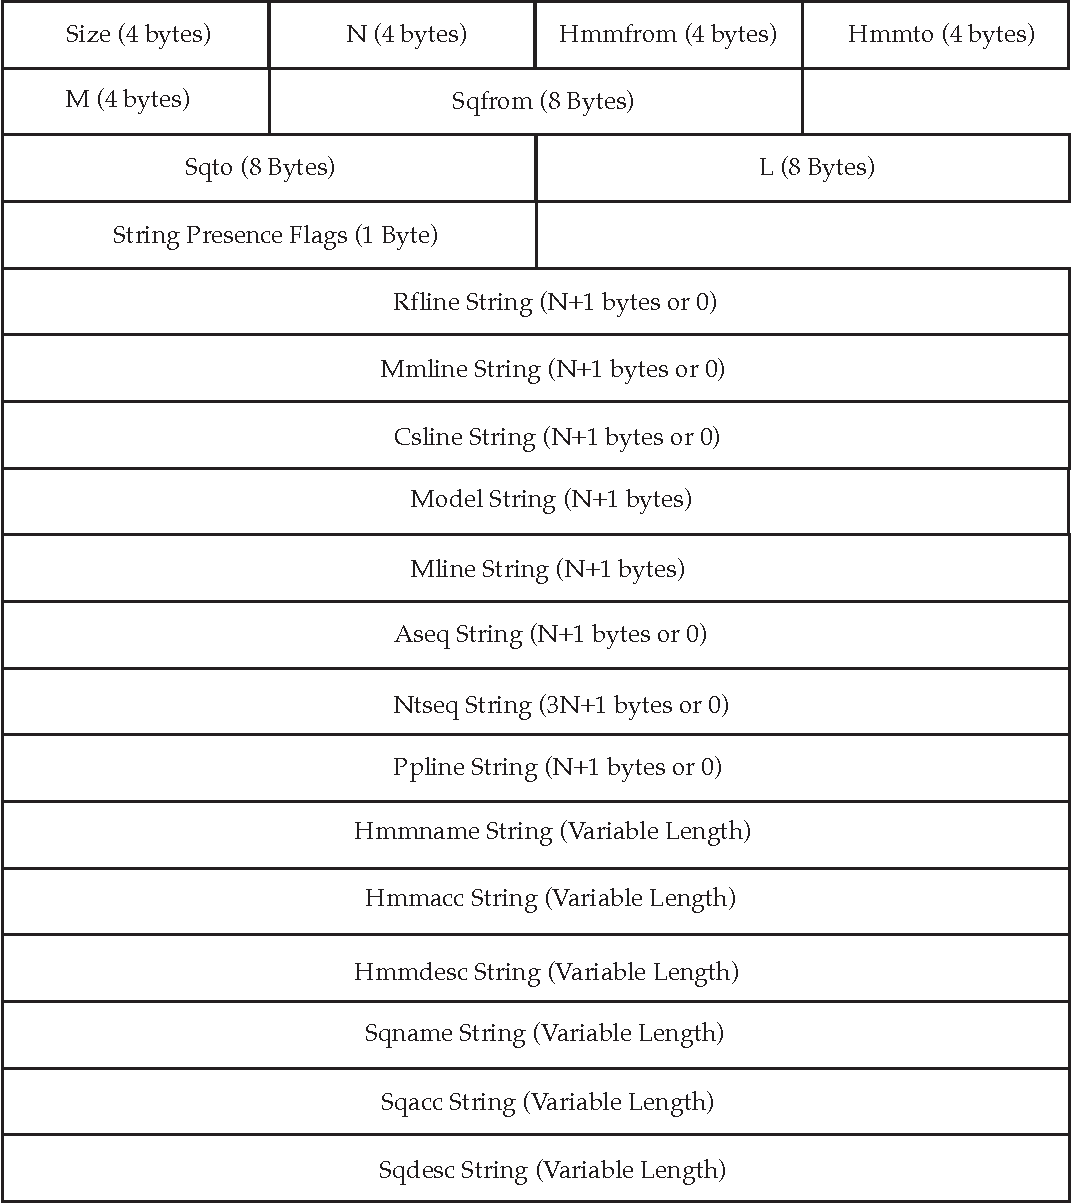
\includegraphics[width=\textwidth]{inclusions/alidisplay-serialize.pdf}
    \caption{Serialized {P7\_ALIDISPLAY} Structure}
    \label{fig:alidisplay-serialize}
  \end{figure*}

The {P7\_ALIDISPLAY} structure (Figure \ref{fig:alidisplay-serialize}) contains a number of variable-length fields, several of which are optional.  The serialized structure begins with a size field containing its length in bytes, followed by the fixed-length fields of the data structure.  A byte of string presence flags encodes the presence or absence of each of the optional field, using a one-hot format.  Then, the variable-length fields of the data structure are serialized as byte arrays.

\begin{adjustwidth}{}{-1in}   
\chapter{Manual Pages Related to the Server}
\input{manpages_server}
\end{adjustwidth}

The server's response to an instruction is similar to its response to a search that causes an error.  It sends an {HMMD\_SEARCH\_STATUS} object that describes the command, followed by a text string.  In the case of a request for the server's contents, the text string specifies the number of databases that the server has available to search, along with a description of each database.  The response to a shutdown instruction indicates whether the shutdown command was accepted or refused due to password miss-match.


\chapter{Acknowledgments}
Simon Potter of the European Bioinformatics Institute was of great help in understanding the daemon's interactions with the EBI's web servers.  We would also like to thank all of the organizations that have supported the development of HMMER, as well as all of the individuals who have contributed to it. In particular, Washington University, the National Institutes of Health, Monsanto, the Howard Hughes Medical Institute, and Harvard University have been major supporters of this work.  For a more thorough set of acknowledgments that includes a discussion of HMMER's history, please see the \underline{HMMER User's Guide}.

\label{manualend}

% To create distributable/gitted 'distilled.bib' from lab's bibtex dbs:
%   # uncomment the {master,lab,books};
%   pdflatex main
%   bibdistill main.aux > distilled.bib
%   # restore the {distilled} 
% 
\nobibliography{distilled}
%\nobibliography{master,lab,books}

\end{document}



